31. а) Раз прямые параллельны, $k=3,6.$ Подставим координаты точки $D:\ 8,2=3,6\cdot(-0,5)+b,\ b=10.$  Построим прямую $y=3,6x+10$ по двум точкам $(0;10)$ и $(-5;-8).$
$$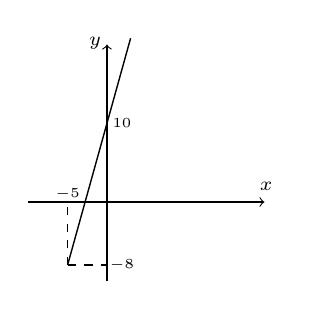
\begin{tikzpicture}[scale=0.1]
\tikzset {line01/.style={line width =0.5pt}}
\tikzset{line02/.style={line width =1pt}}
\tikzset{line03/.style={dashed,line width =0.5pt}}
%\filldraw [black] (0,0) circle (1pt);
\draw [->] (-10,0) -- (20,0);
\draw [->] (0,-10) -- (0,20);
\draw[line01] (-5,-8) -- (3,20.8);
\draw[line03] (-5,-8) -- (0,-8);
\draw[line03] (-5,-8) -- (-5,0);
%\draw[line03] (-1,1) -- (0,1);
%\draw[line03] (-1,0) -- (-1,1);
%\draw[line01] (0,-3) -- (-2,5);
%\draw (0.6,-4) node {\tiny $-4$};
%\draw (-1.6,-0.7) node {\tiny $-1$};
\draw (20.2,2) node {\scriptsize $x$};
\draw (-5,1) node {\tiny $-5$};
\draw (1.9,-8) node {\tiny $-8$};
\draw (1.9,10) node {\tiny $10$};
\draw (-1.5,20.2) node {\scriptsize $y$};
\end{tikzpicture}$$
б) Подходят любые две прямые, одна из которых вертикальна, а другая горизонтальна, например $x=1,\ y=1.$\\
